% Chapter 5
%
\chapter{Experiments and System Evaluation} % Main chapter title
%
\label{Chapter5} % For referencing the chapter elsewhere, use \ref{Chapter4} 
%
%\emph{} = Italic
%TODO review!
This chapter will discuss the experiments done. These will give some insight into what can be expected from the Serverless mode, in the current status. It will also discuss and compare SendIt to other solutions, and evaluate how SendIt matches up against these solutions.
%
\section{Experiments}
In this section the experiments conducted will be discussed. The reasoning behind doing them, the way they were conducted, as well as the results will be discussed. The impact of the results and what the results mean for the usage of SendIt will also be clearly stated and evaluated.
%
\subsection{Motivation and contribution}
%
The experiment original goal of doing the experiment was to see how much time the users of the serverless mode had to do the WebRTC connection offer and answer, from now referred to as the connection setup. The serverless mode requires manual interactions from the users, so knowing the time constraint is important for using the system optimally. In addition, if improvements were to be implemented, it would be necessary to have a benchmark to test against. It would also give a good indication on how to best proceed with improving the solution. As an added bonus, the setup for the experiment can also function as a framework for testing possible improvements and enhancements to the system.

The motivation for doing the experiments was to test the lifetime of the connection setup. Based on the results, the  usability and limitations of the serverless mode would be clear. This indicates the advantages and limitations of the serverless mode, which allows for better decision-making when choosing modes. It also allows for a clear definition of the potential problems with the serverless solution and gives a tangible, concrete frame of reference for improving the solution.
In more detail, the goal of the experiments can be divided in to four parts:
%
\begin{itemize}
	\item Find the approximate lifetime of the Offer
	\item Find the approximate lifetime of the Answer
	\item Find the approximate lifetime of the connection setup
	\item Find the most impactful part of the connection setup
\end{itemize}
%
Since the experiment is meant as a reference and benchmark for SendIts functionality, the setup mimics SendIts connection setup and exchange as much as possible. This means the results of the experiment should be directly transferable to SendIt and the results should reflect what to expect from SendIts current functionality. The results are also similar to the conditions and results experienced when developing and testing SendIt.

%
%
\begin{figure}[th]
  \centering
  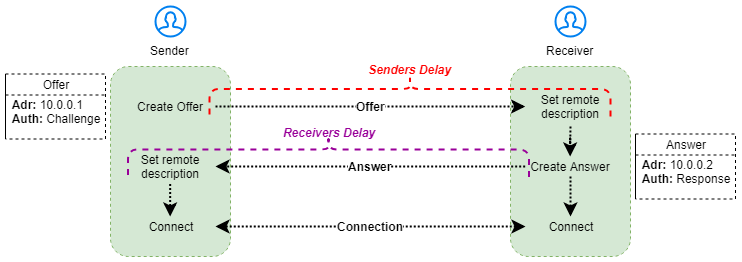
\includegraphics[width=\textwidth]{Figures/Terms}
  \decoRule
  \caption[Experiment terminology]{Simplified illustration of experiment setup}
  \label{fig:terms}
\end{figure}
%
\subsection{Terminology}
%
The terminology is as follows:\\
{\bfseries Offer:} WebRTC connection offer generated by the Sender, to initiate a connection with the receiver.\\
{\bfseries Answer:} WebRTC connection answer generated by the Receiver, from the answer received, to complete the connection setup.\\
{\bfseries Senders delay}(\textit{S}){\bfseries :} is delay from creation of the offer, until it is received by the other endpoint.\\
{\bfseries Receivers delay}(\textit{R}){\bfseries :} is delay from creation of the answer, until it is received by the other endpoint.\\
{\bfseries Split delay:} is the delay split equally between \textit{S} and \textit{R}. If the delay is 10 seconds, it means 5 seconds senders delay and 5 seconds Receivers delay, for a total of 10 seconds delay.
For a better understanding of these terms, look at the simplified representation in \Cref{fig:terms}.
%
%
\subsection{Implementation and results}
In these experiments, the success-rate of connections between a server and a client was measured. The connection was created using WebRTC with a varying delay before the offer and/or answer was shared. The experiments were conducted by having users connect to a web server over HTTP, and naturally having the server deliver content via HTTP. After the necessary HTML and Javascript had been delivered to the client, they would try to establish another connection to the server, using WebSockets. This allows for bi-directional and efficient communication. 
Over this WebSocket connection, the connection setup for the following tests was done. The P2P connection and setup was done utilizing the WebRTC PeerConnection functionality. The whole experiment consisted of three test sets:
%
\begin{itemize}
	\item Test set 1 - Senders delay
	\item Test set 2 - Receivers delay
	\item Test set 3 - Split delay
\end{itemize}
%
Each of these test sets consisted of five tests. Once all test sets were finished (or when the client disconnected), the client shared their log with the server, and the server stored both logs for analysis and comparison. The pattern described below, indicates how one test was done. Once this had been completed for all five tests in all three test sets (for a total of 15 tests) were completed, the experiment was considered finished, and the connection torn down. If a client disconnected before finishing all tests, the results for the tests completed up until that point was shared with the server, and stored.

The tests were done as follows:
For each test, the respective WebRTC offer and answer was exchanged. Depending on the test case, the sharing of the offer or the answer, or both, was delayed by varying length. Once the exchange had completed, the server and the client tried to establish a WebRTC P2P connection. Once this was done, a status check was immediately issued, to check the result of the connection establishment. The results of this status check was used to indicate whether the connection was successful or not.

It is important to note that in initial tests, the results of the status check was noted before trying to utilize the P2P channel to do actual data transfers. In these tests, the result of the status check always correctly indicated whether the connection was successful or not. As such this status check was considered sufficient to indicate the result of the connection establishment. The result of the check was then logged for both server- and client-side. The P2P connection was then torn down and a new connection setup began.
%

For the illustrations in the following sections, the percentage of successful P2P connections is represented on the vertical axis, and the total delay before trying to establish the P2P connection on the horizontal axis. Each test set has a different type of line. 
%
%
\subsubsection*{Experiment 1}
%
\begin{figure}[th]
  \centering
  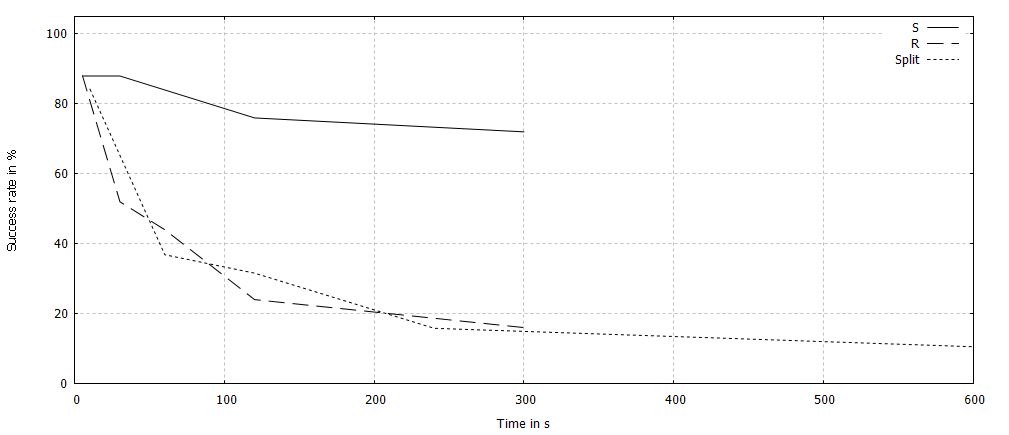
\includegraphics[width=\textwidth]{Figures/Exp1_res}
  \decoRule
  \caption[Experiment 1]{Delayed WebRTC connection setup success rate with Server as Sender (\textit{S})}
  \label{fig:exp1}
\end{figure}
%
The results of the first experiment are shown in \Cref{fig:exp1} The server took the role of Sender in all connections in this experiment.

The size of the dataset is as follows: 25 connections completed test sets \textit{S} and \textit{R}. For Split delay, only 19 connections completed all tests. This is after cleaning the dataset. Connections that failed all tests were removed because the probability of failing all tests and still being a supported connection is very low. These connections are assumed not to be in the target group of computers eligible to use SendIt, and as such would skew the results.

Now lets discuss the findings and implications of this experiment (See \Cref{fig:exp1}). As we can see, \textit{S} is fairly irrelevant. Even at 300 seconds (5 minutes) the success rate is 72\%. \textit{R} is much more important. At a 5 seconds delay, \textit{S} and \textit{R} have the same success rate. However, at 30 seconds, there is a gap of 36\% (\textit{S}=88\%, \textit{R}=52\%). This indicates that the problem with keeping a connection open largely resides on the Receivers end. Splitting the delay equally between \textit{S} and \textit{R} (as indicated by 'Split Delay'), seem to improve connectivity compared to \textit{S}, which corroborates the theory that \textit{S} has more influence on the success rate of creating a connection.

One factor that might influence this result, is that in this experiment the test-server always acted as \textit{S}. The server may have a more stable internet-connection than most endpoints. As such, another experiment was conducted where the server acts as \textit{R}, so the results could be compared and the conclusion re-evaluated.
%
%
\subsubsection*{Experiment 2}
%
\begin{figure}[th]
  \centering
  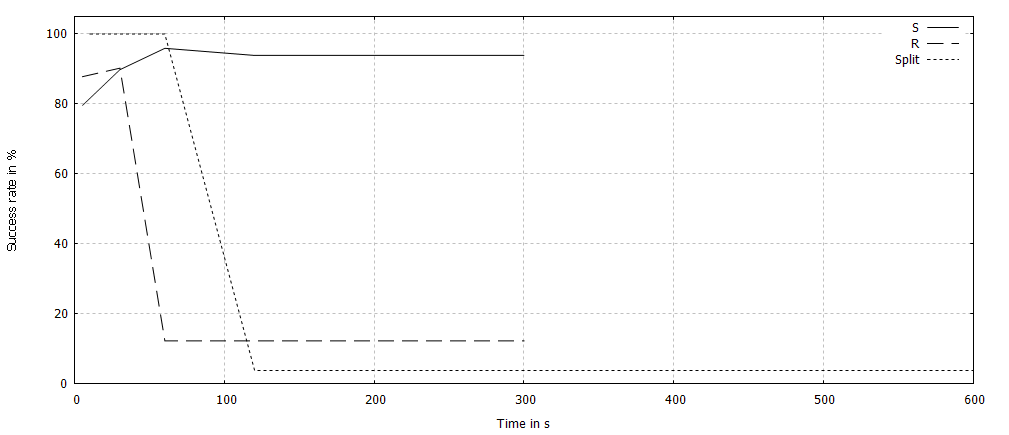
\includegraphics[width=\textwidth]{Figures/Exp2_res}
  \decoRule
  \caption[Experiment 2]{Delayed WebRTC connection setup success rate with Server as Receiver (\textit{R})}
  \label{fig:exp2}
\end{figure}
%
The results of the second experiment are shown in \Cref{fig:exp2} The server took the role of Receiver in all connections in this experiment.

The size of the dataset is as follows: 49 connections completed test set \textit{S}. For test set \textit{R}, 41 connections completed all tests. Finally, for Split delay, 27 connections completed all tests. This is after cleaning the dataset. Connections that failed all tests were removed because the probability of failing all tests and still being a supported connection is very low. These connections are assumed not to be in the target group of computers eligible to use SendIt, and as such would skew the results.

Because of some technical issues during the second experiment, a lot of connections timed out after only completed a few tests. As such, connections who did not complete the first test set (\textit{R}) were also excluded. During analysis of the results, it also became clear that there were a number of repeating connections from the same client, with identical results, in a very short time span. As such, results from the same IP with identical results, with less than one hour between tests, were removed. This resulted in a more correct representation of the data gathered.

Now lets discuss the findings and implications of this experiment (See \Cref{fig:exp2}). In the same vain as in Experiment 1, \textit{S} is much less impactful than \textit{R}. In this experiment, \textit{R} has an even more drastic and rapid decrease in success-rate. Already after 60 seconds, the rate has dropped to only 12\%. \textit{R} on the other hand, experiences very little variation in success-rate over time. It is safe to say that this experiment indicates that \textit{R} is insignificant in comparison to \textit{S}. It is also interesting to note that the Split delay has an even more severe drop-off than \textit{R}. Between 60 and 120 seconds, it drops from 100\% success-rate to only 4\%. Why this is the case is hard to evaluate, as there is no clear indication why this behavior occurs. 
%
%
\subsection{Impact and findings}
%
\begin{figure}[th]
  \centering
  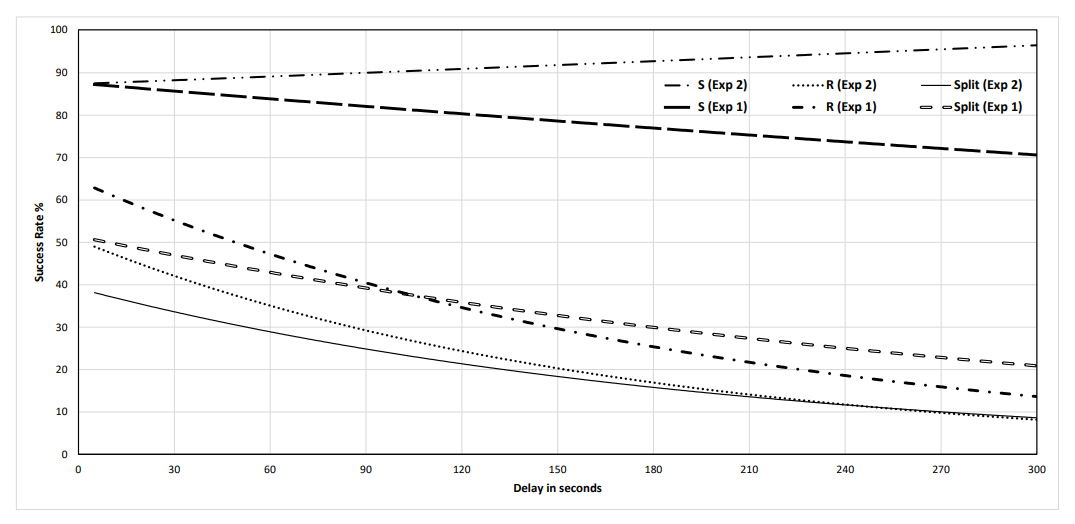
\includegraphics[width=\textwidth]{Figures/Experiment_comp}
  \decoRule
  \caption[Experiment comparison]{Shows the exponential approximation of the results in the two experiments for comparison. These indicate how the average results will look over time.}
  \label{fig:expcomp}
\end{figure}
%
\begin{table}
	\caption[Comparison of Senders delay]{Comparison of the Senders Delay in Experiment 1 and 2. The values represent the rate of success in establishing a connection}
	\label{tab:comp_send}
	\centering
	\begin{tabular}{c@{\qquad}ccccc}
	    \multirow{3}{*}{\raisebox{-\heavyrulewidth}{\textit{S}}} & \multicolumn{5}{c}{Time in seconds}\\
	  	\cmidrule{2-6}
        & 5 & 30 & 60 & 120 & 300\\
        \midrule
        $Experiment~1$ & 88\% & 88\% & 84\% & 76\% & 72\% \\
        $Experiment~2$ & 80\% & 90\% & 96\% & 94\% & 94\% \\
        \bottomrule
	\end{tabular}\\
\end{table}
%
\begin{table}
	\caption[Comparison of Receivers delay]{Comparison of the Receivers delay in Experiment 1 and 2. The values represent the rate of success in establishing a connection}
	\label{tab:comp_recv}
	\centering
	\begin{tabular}{c@{\qquad}ccccc}
		\multirow{3}{*}{\raisebox{-\heavyrulewidth}{\textit{R}}} & \multicolumn{5}{c}{Time in seconds}\\
	  	\cmidrule{2-6}
        & 5 & 30 & 60 & 120 & 300\\
        \midrule
        $Experiment~1$ & 88\% & 52\% & 44\% & 24\% & 16\% \\
        $Experiment~2$ & 90\% & 93\% & 12\% & 12\% & 12\% \\
        \bottomrule
	\end{tabular}\\
\end{table}
%
\begin{table}
	\caption[Comparison of Split delay]{Comparison of the Split delay in Experiment 1 and 2. The values represent the rate of success in establishing a connection}
	\label{tab:comp_split}
	\centering
	\begin{tabular}{c@{\qquad}ccccc}
      	\multirow{3}{*}{\raisebox{-\heavyrulewidth}{Split~delay}} & \multicolumn{5}{c}{Time in seconds}\\
	  	\cmidrule{2-6}
        & 10 & 60 & 120 & 300 & 600\\
        \midrule
        $Experiment~1$ & \textasciitilde88\% & \textasciitilde37\% & \textasciitilde32\% & \textasciitilde16\% & \textasciitilde11\% \\
        $Experiment~2$ & 100\% & 100\% & \textasciitilde4\% & \textasciitilde4\% & \textasciitilde4\% \\
        \bottomrule
	\end{tabular}\\
\end{table}
%
We can now compare the results from these experiments (Shown in  \Cref{tab:comp_send}, \Cref{tab:comp_recv}, \Cref{tab:comp_split} and \Cref{fig:expcomp}), by looking at this data.

As we can see the results are fairly similar. This indicates that delaying the Answer, has far more impact than delaying the Offer. We can assume this, by comparing the success-rate of connections for \textit{R} and \textit{S} in \Cref{tab:comp_send} and \Cref{tab:comp_recv}. We see the percentages drop drastically, as the delay increases for \textit{R}. On the contrary, \textit{S} has only a slight decrease in success-rate (and only for Experiment 1). From this we can conclude that the original assumption was correct: The Answer is by far the most impactful part of the connection setup.

By looking and comparing the results from Experiment 1 and 2, we can clearly identify that \textit{R} experiences a significant drop between 30 and 60 seconds delay. With a success-rate of respectively 52\% and 93\% for 30 second delay, compared to 44\% and 12\% for a 60 second delay. With this knowledge, we can conclude the average lifetime of \textit{R} is somewhere between these to values.

One can also draw the conclusion that the offer can last at least 5 minutes, based on the above experiments. The lowest success-rate for the offer was 72\% at 300 seconds (5 minutes) delay, in experiment 1. For experiment 2, this value was comparatively 94\%. From this it can be extrapolated that it is likely that a connection will be successful, even if \textit{S} approaches, or even extends past 5 minutes.

From the two conclusions above: \textit{S} having a lifetime of at least 5 minutes, and \textit{R} having a lifetime between 30 and 60 seconds, we can combine them to find the average lifetime of the connection setup. Even though \textit{R} experiences a rapid decrease between 30-60 seconds, \textit{S} seems to have the ability to extend past 5 minutes. For this reason, the lifetime of the connection setup will be around 6 minutes. This should be kept in mind, if one is utilizing the serverless mode.

Finally, an interesting observation, however expected, is that when the Server acted as the Receiver (Experiment 2), the results were far more volatile, then when the roles were reversed (Experiment 1). This is probably because it is beneficial to have the most stable endpoint initiate the connection, as it allows for more predictable results.

The more stable connection is likely to have more routes to be reached through, and as such is more likely to result in a more stable setup environment. If the routes changes with the more stable connection being the initiator, one of the other routes can be used instead. This is not the case for unstable, constantly changing connections. It should be emphasized that there is no proof to back up such an assumption in these experiments, but it seems to be the likely scenario.
%
%
\section{Security and system evaluation}
To understand the contribution and usability of SendIt, an analysis of existing solutions is needed. By comparing SendIt with existing solutions it is possible to get an idea of what has been improved, what stayed the same, and what still needs to be worked on. In the following section the e-mail system, a generic SNS system and SendIt will all be evaluated and analyzed.
%
\subsection{Evaluation of SendIt}
%
  SendIt has fewer weaknesses than the other two systems. The main advantage is the direct transfer, which minimizes the attack surface compared to the other two solutions. This evaluation will not include all attacks made possible by the technology chosen, but rather focus on the weaknesses that come as a consequence of the proposed system. By this it is meant that attacks that are present in all JavaScript solutions will not be discussed. If the attack is possible because of the way JavaScript is implemented in this solution, it will be included.
%
  %First trust!!!
  \subsubsection*{First trust}
  %
  The main weakness, as mentioned previously, is the first trust. This can allow an attacker to appear as the legitimate owner of an identity, without this being the case. This is a risk that any user should be aware of, as it is a critical part of the system. Even though it is a part of the design choice, it has to be acknowledged that this is less than optimal.

  The mitigation for such attacks is split in two parts. The first is relying on the user to evaluate whether the user is legitimate. By using social cues, like timing, each user should evaluate if it is likely that the other identity would initiate a transfer. One can also contact the other endpoint and confirm that it is actually them. This is of course only necessary for the first connection.

  The second is the trust model, which is an automatic part of the system. It combats this issue by sharing information and allowing users to have as much data as possible, on all identities. This allows for detection of false identities and will eventually make these identities untrusted entities in the whole system.
%
  \subsubsection*{DHT}
  While P2P transfer is direct communication between two endpoints, it needs some way to set up the connection. Traditionally this has been done using servers or DHT. Since the whole point is to avoid using servers, the only option left is DHT. DHT relies on connecting to specific endpoints, called bootstrapping, to enter the network. This is predictable behavior that can be exploited by attackers, and it also increases the difficulty of using the system.

  As such, the system suggested in this thesis leaves it up to the end users to decide how to share the information, as it is unpredictable and allows for easier usage of the system. It removes the need for any bootstrapping or server, and leaves the decision of the preferred way of sharing the information up to the user.
  
  %ACS!!!
  \subsubsection*{ACS}
  %
  Another attack vector is the ACS service. If it is not trusted, it can pose a security risk, as the endpoint has to rely on the fact that the ACS server relays the data to the correct recipient. If the data sent is encrypted, it will not pose any immediate risk, but it will stop the endpoint from connecting to anyone, as the other endpoint will not get authenticated properly. If it is the first time these endpoints are connecting, however, it puts the victim at risk of being put in touch with the wrong identity.

  The ACS server can also act as a logger that keeps track of which identities are communicating with each other. While not directly an attack, it can raise privacy issues. Since it allows for monitoring of traffic, it can also be argued that it can be used for reconnaissance, which allows for a targeted attack on one of the endpoints. Because of this, endpoints should only use ACS servers they trust.

  %MITM
  The ACS server can also deploy MitM attacks, during the connection setup, which leads to the attacker gaining full access to the data transferred. The biggest problem with this type of attack, is that in most cases it cannot be detected until after the data has already been shared and the attacker has full access to it. It will eventually be detected by the trust system, but at that point it might already be too late. While there is also a possibility for this to happen during the connection setup of the Serverless mode, it is much harder to do, since there is no pre-determined channel for sharing the offer, and as such the attacker has no set point to attack. 
%
  %XSS
  \subsubsection*{Other}
  Finally, there is a theoretical possibility of having XSS attacks executed in the client, since the Serverless mode relies on user input. While there are countermeasures deployed, one can never guarantee that there are no such security holes.

%
%
\subsection{E-mail system comparison}
\label{sec:email_syst}
  %E-mail
  %Anything is an improvement
  Comparing the e-mail system to SendIt is a little like comparing your mailbox to a safe. While the mailbox can be locked and it can be made more secure, it is still outside your house, with no access control, not made to withstand attacks, and ultimately, it can just be stolen as a whole. In contrast the safe is made to withstand attacks, and store your data privately.

  In a similar fashion, e-mail was made to send and receive information, like a mailbox. SendIt is made to make this process secure against outside tampering and allow for minimal risk while exchanging information. To continue the analogy, it is like meeting the Sender with your safe, giving him a small slot to put the mail in, that only fits the letter you expect to receive, and immediately returning back to the safety of your house. To summarize, the email system offers some secure solutions, but guarantees none. In practice that means one should assume that none is applied. As such, anything is an improvement.
%
%
  \subsubsection*{Direct transfer}
  %No temporary storage - direct transfer
  The first major advantage SendIt has over traditional e-mails is that it transfers the file directly. None of the issues stemming from files being stored in transit, applies to SendIt. These issues range from attackers hacking the server and getting access to the files, to allowing attackers to monitor data going through the server, since it will always be routed through. As a general rule, a resource is more secure, the less copies exists, since it limits the attack surface.

  %Files will be broken if given enough time
  Another point to take into consideration is that even if only encrypted data is stored on a server, if an attacker gets access to the data, it is only a question of how long it takes to break the encryption. As such, minimizing the risk of leaking any data should be considered critical. This is why direct transfer of files offer such a big advantages.

  %Lower attack surface - direct transfer (TIME!)
  The attack surface which is exposed is also important to evaluate. Having a server store the files, means the attack surface is quite big, since it is always online. With SendIt's direct transfer function, the file is only available during transfer. The time difference for how long the file is available to be attacked is huge. As such, this is another advantage of direct transfer, since the attack surface is significantly reduced.
%
  \subsubsection*{Authentication}
  %No possibility to impersonate real Sender
  Sender and Receiver guarantee is another big advantage of SendIt. In the e-mail system the Senders identity can be forged easily, which is not the case for SendIt. It also has some issues where the data sent is not kept confidential and can easily be stolen by a passive listening attack. These two combined makes phishing attacks as well as targeted exploits easier to create, since you know what data or information the endpoint is seeking or expecting. By sending this data from a forged address, the chances of successful attacks increase. The e-mail system have S/MIME which allows for authentication, but as discussed in \Cref{sec:intro_email}, it is rarely used and not user friendly.
  %
  \subsubsection*{Content control}
  %All content received
  In the ordinary e-mail system, one is also not able to decide which content to receive or not. If someone sends an e-mail attachment, it will be delivered to the receiver's PC, or at least their e-mail server. This is unfortunate, since receiving malicious files may cause them to be executed at a later time, or by a unintended action. It is also possible that they may execute without the user knowingly doing so. As such, it is optimal for the user to be able to stop the transfer of unwanted files, like SendIt supports.
  %Automated spreading
  Automatic spreading of malicious files is a big problem today. It is spread to all the victims contacts and keeps spreading in a similar fashion. While SendIt has no direct solution to mitigate this, the fact that it does not support multicast, and that the files cannot be automatically received, will naturally take care of resolving this issue.
%
%
  \subsubsection*{Connection setup}
  % - Needs connection setup
  The disadvantage of SendIt is that it is required to complete a connection setup phase in order to communicate with the other endpoint. The e-mail system has no such need and one can easily transfer information at any time without the user having to worry about the connection setup. This is because all communication occurs between the client and a server that is publicly available.
%
  \subsubsection*{Synchronous connection}
  % - Synchronous
  Another case where SendIt exhibits different behavior is during the actual transfer. While the advantages of direct transfers have been clearly indicated, SendIt does lack support for asynchronous transfers. This is a point where the regular e-mail solution has the edge over SendIt. It can be argued, however, that it is a small obstacle to overcome, for such an increase in security.
%
  \subsubsection*{First trust}
  % - First trust
  Finally, the e-mail system does not have to rely on the trusted first setup, that SendIt does. In the case that the e-mail system uses the security features available, it relies on PKI for the initial trust. This choice of a central service makes sense in the e-mail system which relies on servers, but not for SendIt.
%
  %
\subsection{SNS and Cloud systems comparison}
  %SNS
  While there is no one SNS or cloud based system to compare against, they all share certain functionality and design choices. As such this generalization will be the model used for comparison. In order to avoid re-iterating the same point as in the \emph{Direct transfer} section above (\Cref{sec:email_syst}), this applies equally to SNS and Cloud based systems. This is why SendIt provides a clear use case and improvement to current systems.
  %No temporary storage - direct transfer
  %Files will be broken if given enough time
  %Lower attack surface - direct transfer (TIME!)
%
  \subsubsection*{False E2E encryption}
  %'E2E encryption' not real - skype!
  As mentioned in \Cref{sec:cloudetc} and shown in \Cref{fig:sns}, false E2E encryption is sometimes utilized in these systems. It is scary as a consumer of these services, because both you and your communication partner are unable to verify if the communication has true E2E encryption or not. Effectively this is a MitM attack by design. As such, when using these services, one should assume that the data can be decrypted and read by the service and whoever they disclose the data to. For SendIt, the public key cryptography guarantees end to end encryption, since they are exchanged over P2P, which means no central service can tamper with the key sent. 
%
  \subsubsection*{Identity swapping}
  %Hard to switch identities
  Another thing that is hard to do in these systems is swap identities, if the user desires. One may not want to associate an identity with both work and private life, which means the need for several identities arises. This requires logging in and out, managing two sets of credentials and keeping track of which identity is currently in use. For SendIt all the user has to do is swap to the file containing the correct keys and the identity has been changed.
%
  \subsubsection*{Other}
  The points where SNS and Cloud based systems have clear advantages also resembles that of the e-mail system. The points made in the sections \emph{Connection setup} and \emph{First trust} in \Cref{sec:email_syst} apply to these systems as well. For the first trust in these systems, they also rely on the PKI model, which makes sense since they are based around the server-client model as well.

  These solutions do have the advantage of storing a backup of your files, which can be desired in certain situations. This can easily be achieved after transfer though, and gives the user more control over how it is stored. As such, these solutions are more suited for regular files, not files with high requirements in regard to privacy and security.
  % - Needs connection setup
  % - First trust
%